\chapter{Stand van zaken}
\label{ch:stand-van-zaken}

% Tip: Begin elk hoofdstuk met een paragraaf inleiding die beschrijft hoe
% dit hoofdstuk past binnen het geheel van de bachelorproef. Geef in het
% bijzonder aan wat de link is met het vorige en volgende hoofdstuk.

% Pas na deze inleidende paragraaf komt de eerste sectiehoofding.

In dit hoofdstuk wordt de stand van zaken besproken wat tabeltransformatie van afbeeldingen betreft. Er wordt besproken wat tabulair data is, waarom tabellen belangrijk zijn in de huidige informatiewereld, wat er bedoeld wordt met tabeldetectie en structuuranalyse, waar de uitdagingen hierbij zich bevinden en tenslotte wordt er in detail de verschillende technieken besproken die ontwikkeld werden om tabellen te kunnen detecteren en analyseren, met hun voor- en nadelen.

\section{Tabulair data}
\label{sec:tabulair-data}

\subsection{Definitie}
\label{subsec:definitie-tabulair-data}

Zoals \textcite{Zanibbi2003} het aangeeft, is een tabel een vorm van visualiatie dat men gebruikt om ermee data op te zoeken en te vergelijken. Meer specifiek geeft, volgens \textcite{Zanibbi2003}, een tabel indexeringschema's weer voor relaties. Een relatie heeft een verzameling van $\eta$ \glspl{tupel}, die de domeinen of dimensies van de relatie genoemd worden.

De dimensies kunnen d.m.v. verschillende combinaties van rijen en kolommen opgesteld worden, waardoor verschillende tabelopstellingen exact dezelfde informatie op verschillenden manieren kunnne weergeven. Dit kan gedemonstreerd worden a.d.h.v. de volgende twee figuren.

\begin{figure}[H]
    \centering
    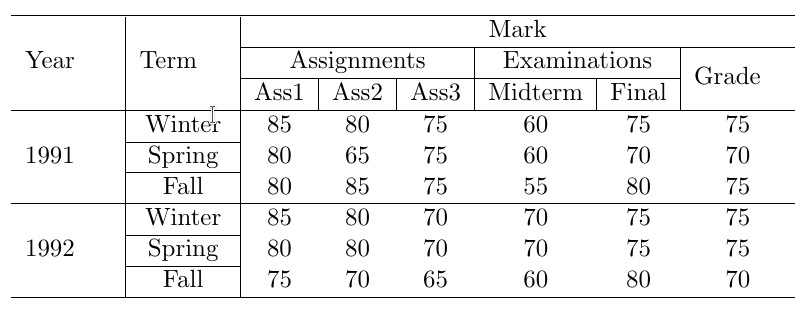
\includegraphics[width=0.8\textwidth]{img/tabel_verschillende_opstelling_dezelfde_data_1.png}
    \caption{Een tabel van evaluaties. Het geeft dezelfde informatie weer als tabelfiguur \ref{fig:tabel_verschillende_opstelling_dezelfde_data_2}. Bron: \cite{Long2010}}
    \label{fig:tabel_verschillende_opstelling_dezelfde_data_1}
\end{figure}

\begin{figure}[H]
    \centering
    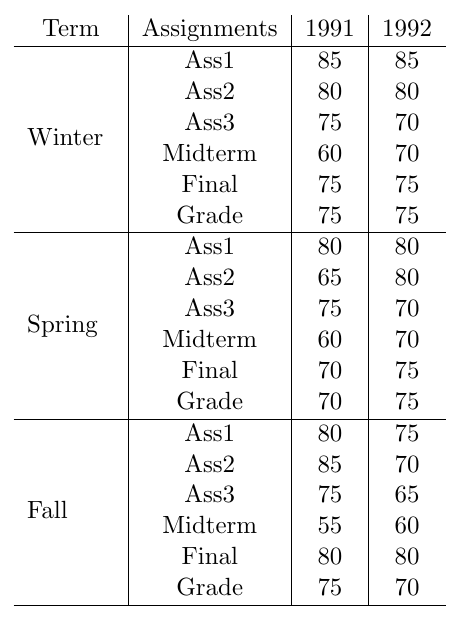
\includegraphics[width=0.5\textwidth]{img/tabel_verschillende_opstelling_dezelfde_data_2.png}
    \caption{Een tabel van evaluaties. Het geeft dezelfde informatie weer als tabelfiguur \ref{fig:tabel_verschillende_opstelling_dezelfde_data_1}. Bron: \cite{Long2010}}
    \label{fig:tabel_verschillende_opstelling_dezelfde_data_2}
\end{figure}

Hoewel beide tabellen identiek zijn wat informatieinhoud betreft, kan duidelijk gemerkt worden dat tabelfiguur \ref{fig:tabel_verschillende_opstelling_dezelfde_data_1} de evaluaties duidelijker weergeeft. Meestal wordt een combinatie van rijen en kolommen zodanig gekozen zodat de data van de tabel zo eenvoudig en snel mogelijk gelezen en geïnterpreteerd kan worden. Ook kunnen verschillende lettertypes, kleuren en lettergroottes gebruikt worden om de leesbaarheid te vergroten.

\subsection{Anatomie}
\label{subsec:anatomie}

\raggedbottom

Volgens \textcite{Wang1996} is een tabel, door \textit{stub scheiding} en \textit{boxhead scheiding}, verdeeld in vier hoofdregio's die in onderstaande figuur \ref{fig:tabel_anatomie} merkbaar zijn. De regio linksbeneden die de rijhoofdingen bevat en de regio rechtsboven die de kolomhoofdingen bevat, worden respectievelijk de \textit{stub} en de \textit{boxhead} genoemd. De regio linksboven, die de categorieën in de \textit{stub} inhouden is gekend als de \textit{stub head} en de \textit{body} tenslotte, is de regio rechts van de \textit{sub} en onder de \textit{boxhead} die de tabeldata-elementen bevat. De snijpunt van een rij en een kolom wordt een \textit{cel} genoemd; en een rechthoekig verzameling van \textit{cellen} is gekend als een \textit{block}.

\begin{figure}[H]
    \centering
    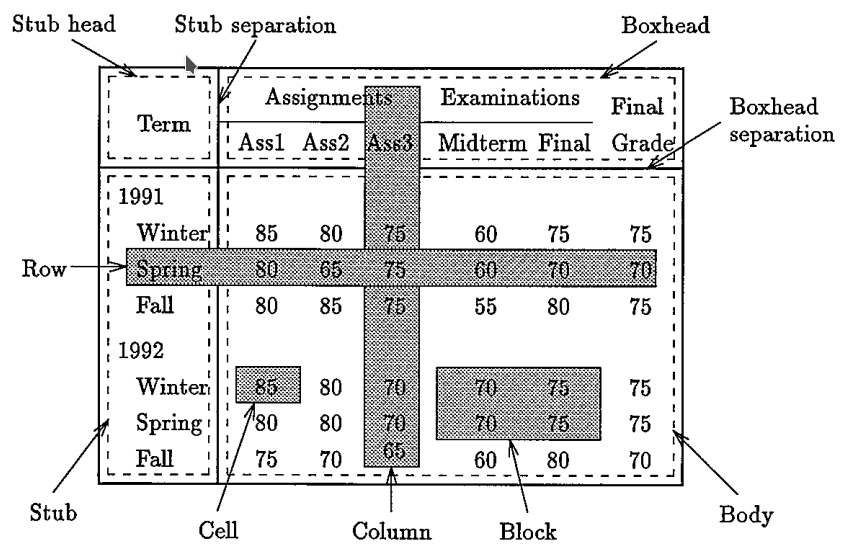
\includegraphics[width=0.8\textwidth]{img/tabel_anatomie.png}
    \caption{De anatomie van de structurele rij-kolomvoorstelling van een tabel. Bron: \cite{Wang1996}}
    \label{fig:tabel_anatomie}
\end{figure}

Zoals men in figuur \ref{fig:tabel_anatomie} kan zien, kunnen multidimensionele relaties in een twee dimensionele tabel gepresenteerd worden door meer dan één categorie te associeren met de \textit{boxhead} en/of met de \textit{stub}. Zo worden hier de rijhoofdingen niet enkel met één hoofdcategorie ``Term`` maar eveneens met meerdere subcategorieën, ``1991`` en ``1992`` geassocieerd. Analoog zijn de kolomhoofdingen gekoppeld aan drie categorieën, namelijk ``Assignments``, ``Examinations`` en ``Finals``.

\subsection{Functie}
\label{subsec:functie}

Als vermeld door \textcite{Shahzad2019}, worden tabellen veelal gebruikt voor het gestructureerd vertonen van essentiële informatie in documenten. Ze worden gebruikt in boeken, artikelen, onderzoekspapers, en verschillende andere soorten media. In sectoren zoals de financiële en de administratieve sectoren wordt data veelal in tabelvorm geformuleerd omdat tabellen, volgens \textcite{Coueasnon2014}, veel informatie voorstellen op een beknopte manier waardoor het begrijpbaar blijft voor de lezer; ze laten ook zo toe de belangrijke delen te benadrukken. 

\subsection{Creatie en representatie}
\label{subsec:creatie-en-representatie}

Doorheen de tijd werden verschillende software applicaties ontwikkeld om digitaal tabulair data aan te maken, te beheren en voor te stellen. Een veelgebruikte software voor tabelcompositie is Microsoft Excel. Het is, zoals \textcite{Wang1996} het vermeldt, een complexe rekenbladprogramma waarbij tabulair data in een werkblad, in een twee dimensionele rooster die a.d.h.v. rij en kolomindexes geadresseerd kan worden, geplaatst wordt.

Een andere bekend software voor het creëren van tabellen is \LaTeX. Het is een systeem voor het zetten van documenten. \textcite{Wang1996} geeft aan dat tabellen in \LaTeX\ gespecifieerd kunnen worden met de ``tabular``- en de ``array``-omgeving. De eerste omgeving wordt meestal gebruikt voor tekstuele tabeldata, de tweede voor wiskundige uitdrukkingen.

Voor de voorstelling van tabellen op het internet, m.a.w. op internetbrowsers, wordt de opmaaktaal HTML gebruikt. Door middel van de ``table``-, ``tr``-, ``th``- en ``td``-tags kunnen tabellen gemaakt en voorgesteld worden.

\section{Tabeltransformatie}
\label{sec:tabel-transformatie}

Verschillende technieken om tabeltransformatie werden reeds ontwikkeld. Echter blijft een algemeen toepasbare oplossing een moeilijk uitdaging, en dit voor diverse redenen.

\begin{itemize}
    \item Tabellen bezitten uiteenlopende layouts en designs, zonder enige standaardisatie
          \autocite{Kasar2014}
    \item Verschillende tabellayouts hebben verschillende features \autocite{Kasar2014}
    \item De typisch kleine inter-klasse variantie tussen tabellen, figuren en grafieken vermoeilijkt
          de detectie van tabellen; de kleine variantie is verantwoordelijk voor de hoge hoeveelheid
          valse positieven bij tabeldetectie \autocite{Embley2006}
  \end{itemize}

\textcite{Kasar2014} beschreeft tabeltransformatie als een proces bestaand uit voornamelijk twee subprocessen: tabeldetectie en tabelstructuuranalyse. 

Met tabeldetectie worden eerst regio's in een bepaalde document geïdentificeerd die overeenkomen met tabellen. Vervolgens wordt tabelstructuuranalyse toegepast om relationele informatie te extraheren van de geïdentificeerde tabelregio's om de logische structuur van de tabellen te achterhalen, zoals bijvoorbeeld de rijhoofdingen, kolommhoofdingen, cellen en meer.

\subsection{Tabeldetectie}
\label{subsec:tabel-detectie}

Tabeldetectietechnieken kan men, kijkend naar de stand van zaken, opdelen in twee klassen: klassieke, op regelgebaseerde algoritmen enerzijds en de recentere, opkomende algoritmen die gebruik maken van machinaal leertechnieken.

\subsubsection{Regelgebaseerde technieken}

\textcite{Watanabe1991} was de auteur van één van de vroegste werken om tabellen te identificeren. De basis voor de tabelidentificatie hier is de identificatie van individuele blokken, ingesloten door horizontale en verticale lijnsegmenten. Eerst worden lijnsegmenten gedetecteerd en hiermee wordt vervolgens de positie van hoekpunten, gevormd door deze lijne, bepaald. Hierna wordt a.d.h.v. de poositie van deze hoekpunten individuele blokken geïdentificeerd. De relatie tussen de verschillende blokken wordt uiteindelijk in globale en individuele boomstructuren gebruikt om te beslissen of het over een tabel gaat of niet.

Het jaar daarop stelde \textcite{Laurentini1992} een methode voor waarbij tekstregio's op een bottom-up manier gedetecteerd worden. De gedetecteerde karakters worden samengebracht tot woorden en deze woorden worden op hun beurt aan elkaar samengevoegd tot tekstblokken. Ook worden de scheidingslijnen gedeteceerd. Voor elke tekstblok wordt diens positie vergeleken met de scheidingslijnen, om te bepalen of het tot een bepaalde tabel behoort.

TINTIN werd door \textcite{Pyreddy1997} voorgesteld, om tabellen te detecteren. Hun algoritme steunt voor de analyse op de extra PDF-metadata van de PDF-documenten.

Enkele jaren later werd het systeem T-Recs, door \textcite{Kieninger2001}, voorgesteld. Het systeem vormt rechthoeken (bounding boxes) voor woorden in het tabel en op een bottom-up manier worden deze bounding boxes gegroepeerd volgens hun logische eenheden. 

\subsubsection{Datagedreven technieken}

\subsection{Tabelstructuuranalyse}
\label{subsec:tabel-structuur-analyse}

\subsection{End-to-end-systemen}
\label{subssec:end-to-end-systemen}
